\documentclass[border=2pt]{standalone}
\usepackage[T1]{fontenc}
\usepackage[scaled=1.0]{helvet}
\renewcommand{\familydefault}{\sfdefault}
\usepackage{sfmath}
\usepackage{amsmath}
\usepackage{xcolor}
\usepackage{tikz}
\usetikzlibrary{positioning,arrows.meta,calc,fit,backgrounds,shapes.geometric}
% palette (light fills, dark strokes: prints well in colour and greyscale)
\definecolor{ink}{HTML}{1F2933}
\definecolor{muted}{HTML}{52606D}
\definecolor{dataS}{HTML}{B7791F}\definecolor{dataF}{HTML}{FDF3E1}
\definecolor{physS}{HTML}{2F6DB5}\definecolor{physF}{HTML}{E6EFFA}
\definecolor{tranS}{HTML}{2E7D4F}\definecolor{tranF}{HTML}{E5F4EA}
\definecolor{repS}{HTML}{6B4FA8}\definecolor{repF}{HTML}{EFEAF8}
\definecolor{greyS}{HTML}{7B8794}\definecolor{greyF}{HTML}{F1F3F5}
\tikzset{
  >={Stealth[length=2.6mm,width=2mm]},
  box/.style={draw, rounded corners=2pt, line width=0.7pt, align=center, inner sep=4pt, text=ink},
  ttl/.style={font=\bfseries\small},
  arr/.style={->, line width=0.9pt, draw=ink},
  darr/.style={->, line width=0.8pt, draw=muted, dashed},
  stage/.style={draw, rounded corners=4pt, line width=0.6pt, dash pattern=on 3pt off 2pt, inner sep=7pt},
  stagelabel/.style={font=\bfseries\small, anchor=south west, inner sep=2pt},
}
\usepackage[none]{hyphenat}
\newcommand{\T}[1]{{\small\bfseries #1}\\[1pt]}

\definecolor{trF}{HTML}{E5F4EA}\definecolor{trS}{HTML}{2E7D4F}
\definecolor{hoF}{HTML}{9D86D6}\definecolor{hoS}{HTML}{5B3FA0}
\definecolor{i0}{HTML}{DCE8F6}\definecolor{i1}{HTML}{B5CDEA}\definecolor{i2}{HTML}{86ADDA}\definecolor{i3}{HTML}{5B8CC8}\definecolor{i4}{HTML}{2F67AE}
\begin{document}
\footnotesize
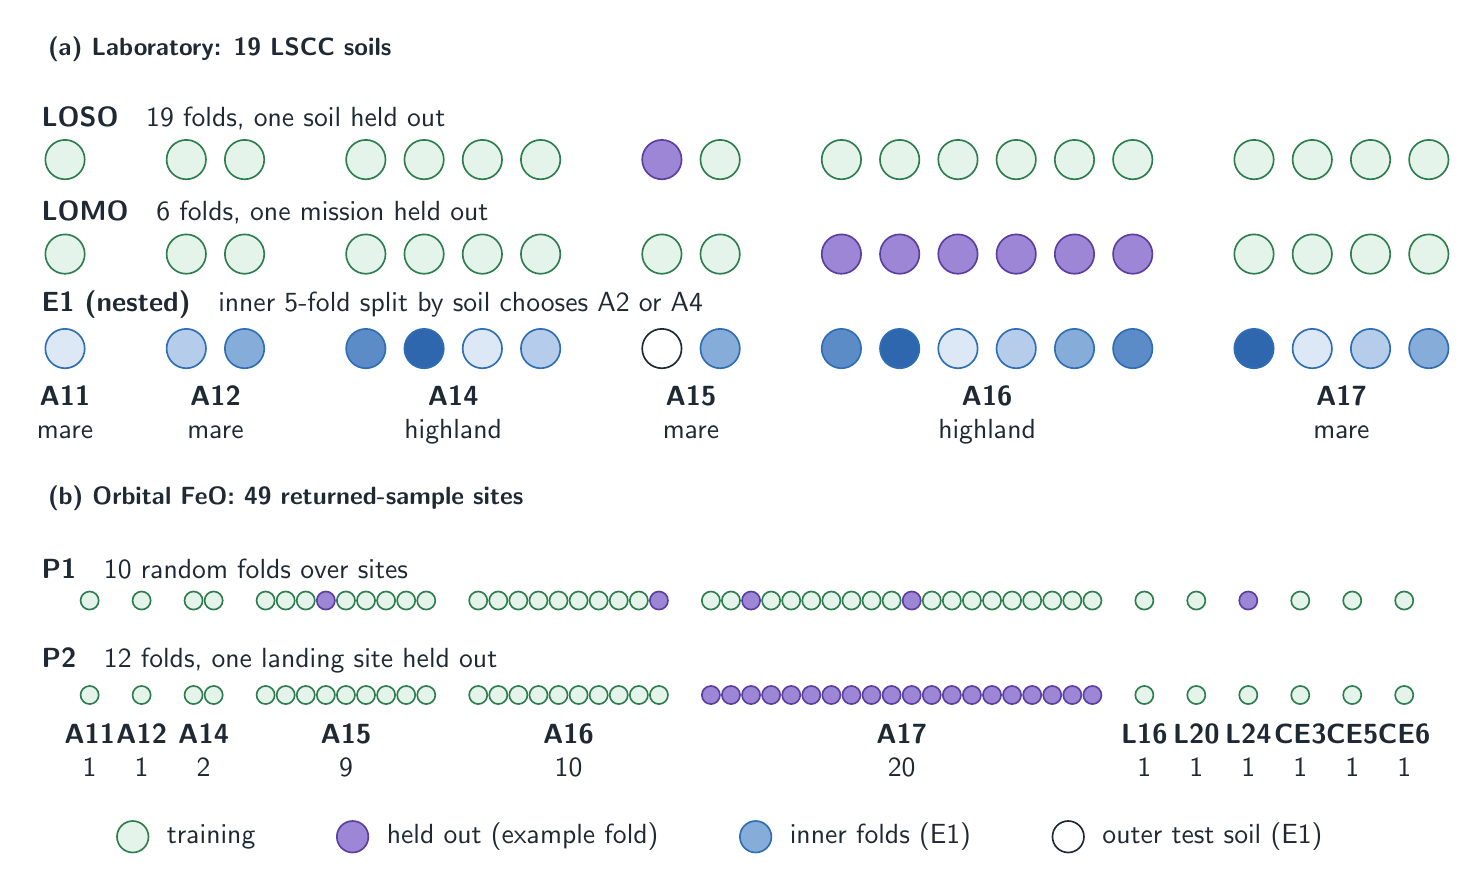
\begin{tikzpicture}[x=1mm,y=1mm]
\tikzset{tr/.style={circle, draw=trS, fill=trF, line width=0.6pt, inner sep=0pt},
         ho/.style={circle, draw=hoS, fill=hoF, line width=0.6pt, inner sep=0pt},
         ot/.style={circle, draw=ink, fill=white, line width=0.6pt, inner sep=0pt},
         rl/.style={anchor=south west, text=ink, inner sep=1pt}}
\node[anchor=west, font=\small\bfseries, text=ink] at (0,14) {(a) Laboratory: 19 LSCC soils};
\node[rl] at (0,3.4) {\textbf{LOSO}\quad 19 folds, one soil held out};
\node[rl] at (0,-8.6) {\textbf{LOMO}\quad 6 folds, one mission held out};
\node[rl] at (0,-20.6) {\textbf{E1 (nested)}\quad inner 5-fold split by soil chooses A2 or A4};
\node[tr, minimum size=5mm] at (3.4,0) {};
\node[tr, minimum size=5mm] at (3.4,-12) {};
\node[circle, draw=physS, fill=i0, line width=0.6pt, inner sep=0pt, minimum size=5mm] at (3.4,-24) {};
\node[tr, minimum size=5mm] at (18.8,0) {};
\node[tr, minimum size=5mm] at (18.8,-12) {};
\node[circle, draw=physS, fill=i1, line width=0.6pt, inner sep=0pt, minimum size=5mm] at (18.8,-24) {};
\node[tr, minimum size=5mm] at (26.2,0) {};
\node[tr, minimum size=5mm] at (26.2,-12) {};
\node[circle, draw=physS, fill=i2, line width=0.6pt, inner sep=0pt, minimum size=5mm] at (26.2,-24) {};
\node[tr, minimum size=5mm] at (41.6,0) {};
\node[tr, minimum size=5mm] at (41.6,-12) {};
\node[circle, draw=physS, fill=i3, line width=0.6pt, inner sep=0pt, minimum size=5mm] at (41.6,-24) {};
\node[tr, minimum size=5mm] at (49,0) {};
\node[tr, minimum size=5mm] at (49,-12) {};
\node[circle, draw=physS, fill=i4, line width=0.6pt, inner sep=0pt, minimum size=5mm] at (49,-24) {};
\node[tr, minimum size=5mm] at (56.4,0) {};
\node[tr, minimum size=5mm] at (56.4,-12) {};
\node[circle, draw=physS, fill=i0, line width=0.6pt, inner sep=0pt, minimum size=5mm] at (56.4,-24) {};
\node[tr, minimum size=5mm] at (63.8,0) {};
\node[tr, minimum size=5mm] at (63.8,-12) {};
\node[circle, draw=physS, fill=i1, line width=0.6pt, inner sep=0pt, minimum size=5mm] at (63.8,-24) {};
\node[ho, minimum size=5mm] at (79.2,0) {};
\node[tr, minimum size=5mm] at (79.2,-12) {};
\node[ot, minimum size=5mm] at (79.2,-24) {};
\node[tr, minimum size=5mm] at (86.6,0) {};
\node[tr, minimum size=5mm] at (86.6,-12) {};
\node[circle, draw=physS, fill=i2, line width=0.6pt, inner sep=0pt, minimum size=5mm] at (86.6,-24) {};
\node[tr, minimum size=5mm] at (102,0) {};
\node[ho, minimum size=5mm] at (102,-12) {};
\node[circle, draw=physS, fill=i3, line width=0.6pt, inner sep=0pt, minimum size=5mm] at (102,-24) {};
\node[tr, minimum size=5mm] at (109.4,0) {};
\node[ho, minimum size=5mm] at (109.4,-12) {};
\node[circle, draw=physS, fill=i4, line width=0.6pt, inner sep=0pt, minimum size=5mm] at (109.4,-24) {};
\node[tr, minimum size=5mm] at (116.8,0) {};
\node[ho, minimum size=5mm] at (116.8,-12) {};
\node[circle, draw=physS, fill=i0, line width=0.6pt, inner sep=0pt, minimum size=5mm] at (116.8,-24) {};
\node[tr, minimum size=5mm] at (124.2,0) {};
\node[ho, minimum size=5mm] at (124.2,-12) {};
\node[circle, draw=physS, fill=i1, line width=0.6pt, inner sep=0pt, minimum size=5mm] at (124.2,-24) {};
\node[tr, minimum size=5mm] at (131.6,0) {};
\node[ho, minimum size=5mm] at (131.6,-12) {};
\node[circle, draw=physS, fill=i2, line width=0.6pt, inner sep=0pt, minimum size=5mm] at (131.6,-24) {};
\node[tr, minimum size=5mm] at (139,0) {};
\node[ho, minimum size=5mm] at (139,-12) {};
\node[circle, draw=physS, fill=i3, line width=0.6pt, inner sep=0pt, minimum size=5mm] at (139,-24) {};
\node[tr, minimum size=5mm] at (154.4,0) {};
\node[tr, minimum size=5mm] at (154.4,-12) {};
\node[circle, draw=physS, fill=i4, line width=0.6pt, inner sep=0pt, minimum size=5mm] at (154.4,-24) {};
\node[tr, minimum size=5mm] at (161.8,0) {};
\node[tr, minimum size=5mm] at (161.8,-12) {};
\node[circle, draw=physS, fill=i0, line width=0.6pt, inner sep=0pt, minimum size=5mm] at (161.8,-24) {};
\node[tr, minimum size=5mm] at (169.2,0) {};
\node[tr, minimum size=5mm] at (169.2,-12) {};
\node[circle, draw=physS, fill=i1, line width=0.6pt, inner sep=0pt, minimum size=5mm] at (169.2,-24) {};
\node[tr, minimum size=5mm] at (176.6,0) {};
\node[tr, minimum size=5mm] at (176.6,-12) {};
\node[circle, draw=physS, fill=i2, line width=0.6pt, inner sep=0pt, minimum size=5mm] at (176.6,-24) {};
\node[align=center, text=ink, anchor=north] at (3.4,-27.5) {\textbf{A11}\\mare};
\node[align=center, text=ink, anchor=north] at (22.5,-27.5) {\textbf{A12}\\mare};
\node[align=center, text=ink, anchor=north] at (52.7,-27.5) {\textbf{A14}\\highland};
\node[align=center, text=ink, anchor=north] at (82.9,-27.5) {\textbf{A15}\\mare};
\node[align=center, text=ink, anchor=north] at (120.5,-27.5) {\textbf{A16}\\highland};
\node[align=center, text=ink, anchor=north] at (165.5,-27.5) {\textbf{A17}\\mare};
\node[anchor=west, font=\small\bfseries, text=ink] at (0,-43) {(b) Orbital FeO: 49 returned-sample sites};
\node[rl] at (0,-53.6) {\textbf{P1}\quad 10 random folds over sites};
\node[rl] at (0,-65.6) {\textbf{P2}\quad 12 folds, one landing site held out};
\node[tr, minimum size=2.3mm] at (6.525,-56) {};
\node[tr, minimum size=2.3mm] at (6.525,-68) {};
\node[align=center, text=ink, anchor=north] at (6.525,-70.5) {\textbf{A11}\\1};
\node[tr, minimum size=2.3mm] at (13.125,-56) {};
\node[tr, minimum size=2.3mm] at (13.125,-68) {};
\node[align=center, text=ink, anchor=north] at (13.125,-70.5) {\textbf{A12}\\1};
\node[tr, minimum size=2.3mm] at (19.725,-56) {};
\node[tr, minimum size=2.3mm] at (19.725,-68) {};
\node[tr, minimum size=2.3mm] at (22.275,-56) {};
\node[tr, minimum size=2.3mm] at (22.275,-68) {};
\node[align=center, text=ink, anchor=north] at (21,-70.5) {\textbf{A14}\\2};
\node[tr, minimum size=2.3mm] at (28.875,-56) {};
\node[tr, minimum size=2.3mm] at (28.875,-68) {};
\node[tr, minimum size=2.3mm] at (31.425,-56) {};
\node[tr, minimum size=2.3mm] at (31.425,-68) {};
\node[tr, minimum size=2.3mm] at (33.975,-56) {};
\node[tr, minimum size=2.3mm] at (33.975,-68) {};
\node[ho, minimum size=2.3mm] at (36.525,-56) {};
\node[tr, minimum size=2.3mm] at (36.525,-68) {};
\node[tr, minimum size=2.3mm] at (39.075,-56) {};
\node[tr, minimum size=2.3mm] at (39.075,-68) {};
\node[tr, minimum size=2.3mm] at (41.625,-56) {};
\node[tr, minimum size=2.3mm] at (41.625,-68) {};
\node[tr, minimum size=2.3mm] at (44.175,-56) {};
\node[tr, minimum size=2.3mm] at (44.175,-68) {};
\node[tr, minimum size=2.3mm] at (46.725,-56) {};
\node[tr, minimum size=2.3mm] at (46.725,-68) {};
\node[tr, minimum size=2.3mm] at (49.275,-56) {};
\node[tr, minimum size=2.3mm] at (49.275,-68) {};
\node[align=center, text=ink, anchor=north] at (39.075,-70.5) {\textbf{A15}\\9};
\node[tr, minimum size=2.3mm] at (55.875,-56) {};
\node[tr, minimum size=2.3mm] at (55.875,-68) {};
\node[tr, minimum size=2.3mm] at (58.425,-56) {};
\node[tr, minimum size=2.3mm] at (58.425,-68) {};
\node[tr, minimum size=2.3mm] at (60.975,-56) {};
\node[tr, minimum size=2.3mm] at (60.975,-68) {};
\node[tr, minimum size=2.3mm] at (63.525,-56) {};
\node[tr, minimum size=2.3mm] at (63.525,-68) {};
\node[tr, minimum size=2.3mm] at (66.075,-56) {};
\node[tr, minimum size=2.3mm] at (66.075,-68) {};
\node[tr, minimum size=2.3mm] at (68.625,-56) {};
\node[tr, minimum size=2.3mm] at (68.625,-68) {};
\node[tr, minimum size=2.3mm] at (71.175,-56) {};
\node[tr, minimum size=2.3mm] at (71.175,-68) {};
\node[tr, minimum size=2.3mm] at (73.725,-56) {};
\node[tr, minimum size=2.3mm] at (73.725,-68) {};
\node[tr, minimum size=2.3mm] at (76.275,-56) {};
\node[tr, minimum size=2.3mm] at (76.275,-68) {};
\node[ho, minimum size=2.3mm] at (78.825,-56) {};
\node[tr, minimum size=2.3mm] at (78.825,-68) {};
\node[align=center, text=ink, anchor=north] at (67.35,-70.5) {\textbf{A16}\\10};
\node[tr, minimum size=2.3mm] at (85.425,-56) {};
\node[ho, minimum size=2.3mm] at (85.425,-68) {};
\node[tr, minimum size=2.3mm] at (87.975,-56) {};
\node[ho, minimum size=2.3mm] at (87.975,-68) {};
\node[ho, minimum size=2.3mm] at (90.525,-56) {};
\node[ho, minimum size=2.3mm] at (90.525,-68) {};
\node[tr, minimum size=2.3mm] at (93.075,-56) {};
\node[ho, minimum size=2.3mm] at (93.075,-68) {};
\node[tr, minimum size=2.3mm] at (95.625,-56) {};
\node[ho, minimum size=2.3mm] at (95.625,-68) {};
\node[tr, minimum size=2.3mm] at (98.175,-56) {};
\node[ho, minimum size=2.3mm] at (98.175,-68) {};
\node[tr, minimum size=2.3mm] at (100.725,-56) {};
\node[ho, minimum size=2.3mm] at (100.725,-68) {};
\node[tr, minimum size=2.3mm] at (103.275,-56) {};
\node[ho, minimum size=2.3mm] at (103.275,-68) {};
\node[tr, minimum size=2.3mm] at (105.825,-56) {};
\node[ho, minimum size=2.3mm] at (105.825,-68) {};
\node[tr, minimum size=2.3mm] at (108.375,-56) {};
\node[ho, minimum size=2.3mm] at (108.375,-68) {};
\node[ho, minimum size=2.3mm] at (110.925,-56) {};
\node[ho, minimum size=2.3mm] at (110.925,-68) {};
\node[tr, minimum size=2.3mm] at (113.475,-56) {};
\node[ho, minimum size=2.3mm] at (113.475,-68) {};
\node[tr, minimum size=2.3mm] at (116.025,-56) {};
\node[ho, minimum size=2.3mm] at (116.025,-68) {};
\node[tr, minimum size=2.3mm] at (118.575,-56) {};
\node[ho, minimum size=2.3mm] at (118.575,-68) {};
\node[tr, minimum size=2.3mm] at (121.125,-56) {};
\node[ho, minimum size=2.3mm] at (121.125,-68) {};
\node[tr, minimum size=2.3mm] at (123.675,-56) {};
\node[ho, minimum size=2.3mm] at (123.675,-68) {};
\node[tr, minimum size=2.3mm] at (126.225,-56) {};
\node[ho, minimum size=2.3mm] at (126.225,-68) {};
\node[tr, minimum size=2.3mm] at (128.775,-56) {};
\node[ho, minimum size=2.3mm] at (128.775,-68) {};
\node[tr, minimum size=2.3mm] at (131.325,-56) {};
\node[ho, minimum size=2.3mm] at (131.325,-68) {};
\node[tr, minimum size=2.3mm] at (133.875,-56) {};
\node[ho, minimum size=2.3mm] at (133.875,-68) {};
\node[align=center, text=ink, anchor=north] at (109.65,-70.5) {\textbf{A17}\\20};
\node[tr, minimum size=2.3mm] at (140.475,-56) {};
\node[tr, minimum size=2.3mm] at (140.475,-68) {};
\node[align=center, text=ink, anchor=north] at (140.475,-70.5) {\textbf{L16}\\1};
\node[tr, minimum size=2.3mm] at (147.075,-56) {};
\node[tr, minimum size=2.3mm] at (147.075,-68) {};
\node[align=center, text=ink, anchor=north] at (147.075,-70.5) {\textbf{L20}\\1};
\node[ho, minimum size=2.3mm] at (153.675,-56) {};
\node[tr, minimum size=2.3mm] at (153.675,-68) {};
\node[align=center, text=ink, anchor=north] at (153.675,-70.5) {\textbf{L24}\\1};
\node[tr, minimum size=2.3mm] at (160.275,-56) {};
\node[tr, minimum size=2.3mm] at (160.275,-68) {};
\node[align=center, text=ink, anchor=north] at (160.275,-70.5) {\textbf{CE3}\\1};
\node[tr, minimum size=2.3mm] at (166.875,-56) {};
\node[tr, minimum size=2.3mm] at (166.875,-68) {};
\node[align=center, text=ink, anchor=north] at (166.875,-70.5) {\textbf{CE5}\\1};
\node[tr, minimum size=2.3mm] at (173.475,-56) {};
\node[tr, minimum size=2.3mm] at (173.475,-68) {};
\node[align=center, text=ink, anchor=north] at (173.475,-70.5) {\textbf{CE6}\\1};
\node[tr, minimum size=4mm] (k1) at (12,-86) {};
\node[anchor=west, text=ink] (t1) at ($(k1.east)+(1mm,0)$) {training};
\node[ho, minimum size=4mm, right=9mm of t1] (k2) {};
\node[anchor=west, text=ink] (t2) at ($(k2.east)+(1mm,0)$) {held out (example fold)};
\node[circle, draw=physS, fill=i2, line width=0.6pt, inner sep=0pt, minimum size=4mm, right=9mm of t2] (k3) {};
\node[anchor=west, text=ink] (t3) at ($(k3.east)+(1mm,0)$) {inner folds (E1)};
\node[ot, minimum size=4mm, right=9mm of t3] (k4) {};
\node[anchor=west, text=ink] (t4) at ($(k4.east)+(1mm,0)$) {outer test soil (E1)};
\end{tikzpicture}
\end{document}